\documentclass[tikz,border=10pt]{standalone}
\usetikzlibrary{shapes.geometric, arrows}

% Define styles for blocks and arrows
\tikzstyle{startstop} = [rectangle, rounded corners, minimum width=3cm, minimum height=1cm,text centered, draw=black, fill=red!30]
\tikzstyle{process} = [rectangle, minimum width=3cm, minimum height=1cm, text centered, draw=black, fill=blue!30]
\tikzstyle{subprocess} = [rectangle, minimum width=2.5cm, minimum height=0.8cm, text centered, draw=black, fill=cyan!20]
\tikzstyle{arrow} = [thick,->,>=stealth]

\begin{document}

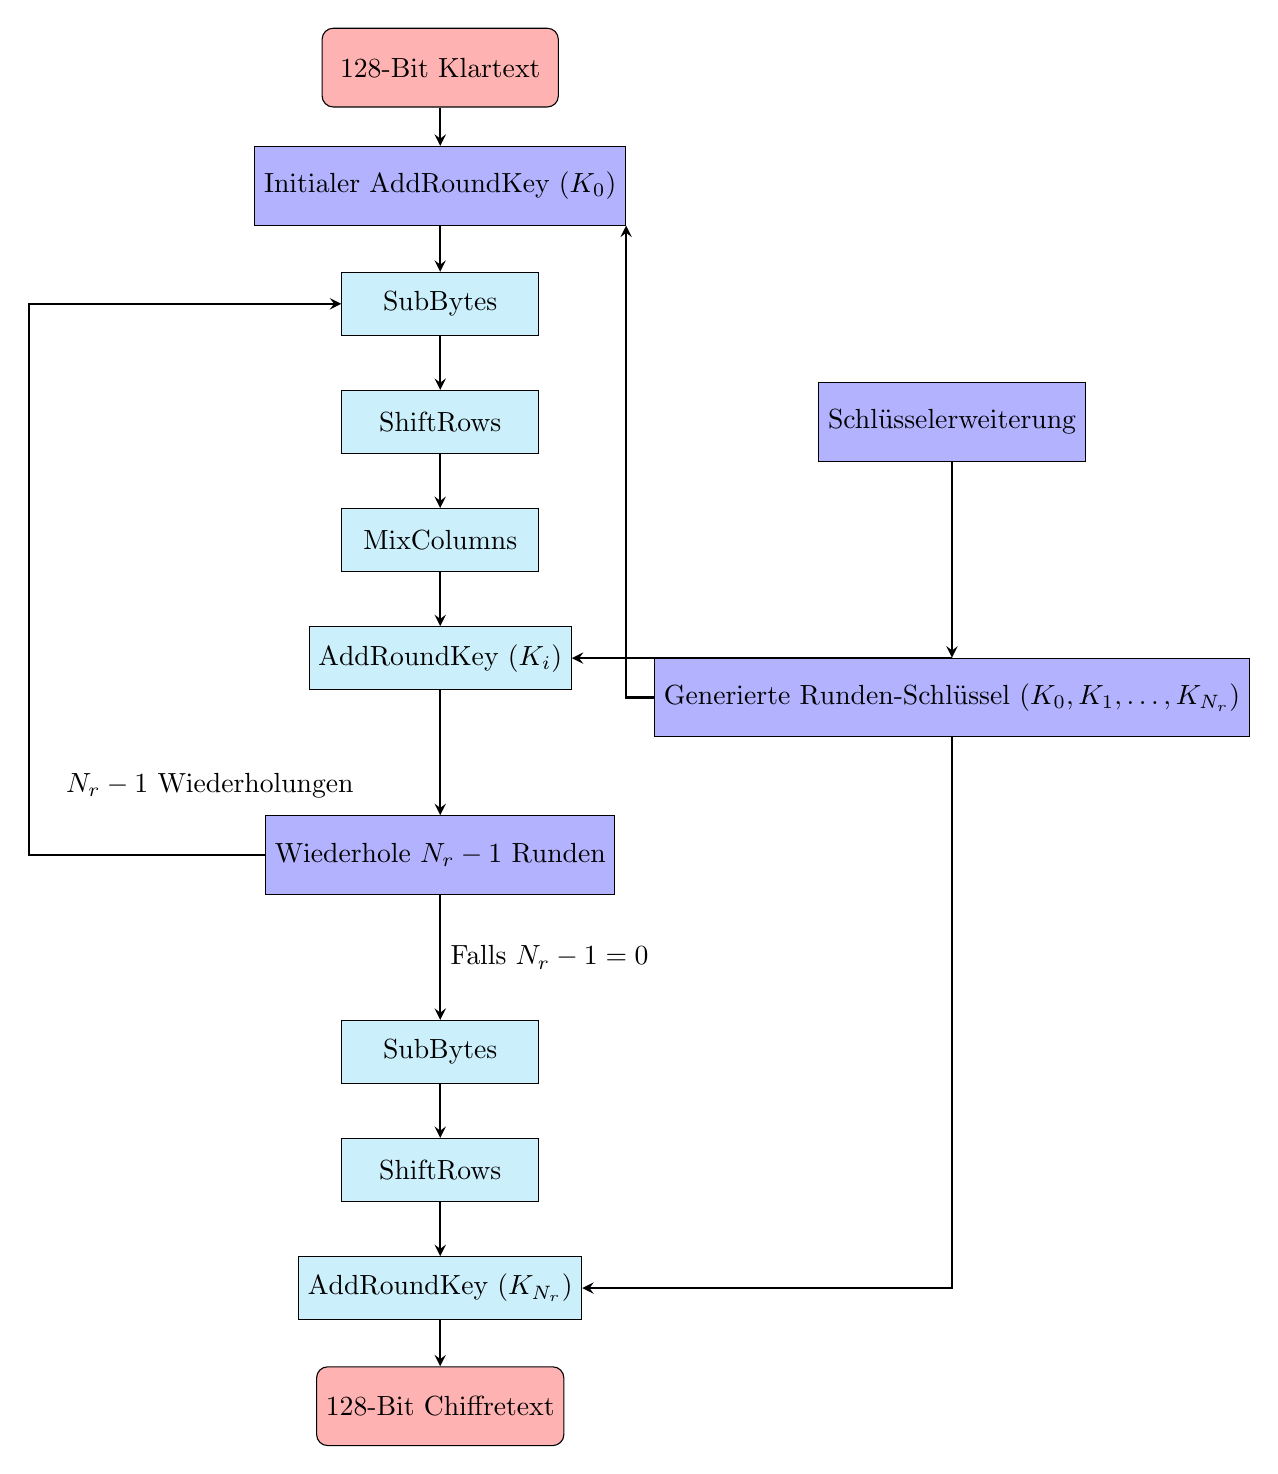
\begin{tikzpicture}[node distance=1.5cm]
    % Nodes
    \node (start) [startstop] {128-Bit Klartext};
    \node (addkey0) [process, below of=start] {Initialer AddRoundKey ($K_0$)};

    % Round structure
    \node (subbytes) [subprocess, below of=addkey0] {SubBytes};
    \node (shiftrows) [subprocess, below of=subbytes] {ShiftRows};
    \node (mixcolumns) [subprocess, below of=shiftrows] {MixColumns};
    \node (addroundkey) [subprocess, below of=mixcolumns] {AddRoundKey ($K_i$)};

    % Loop for Nr-1 rounds
    \node (repeat) [process, below of=addroundkey, yshift=-1cm] {Wiederhole $N_r-1$ Runden};

    % Final round structure
    \node (finalsubbytes) [subprocess, below of=repeat, yshift=-1cm] {SubBytes};
    \node (finalshiftrows) [subprocess, below of=finalsubbytes] {ShiftRows};
    \node (finaladdkey) [subprocess, below of=finalshiftrows] {AddRoundKey ($K_{N_r}$)};
    \node (output) [startstop, below of=finaladdkey] {128-Bit Chiffretext};

    % Key expansion
    \node (keyexpansion) [process, right of=addkey0, xshift=5cm, yshift=-3cm] {Schlüsselerweiterung};
    \node (keys) [process, below of=keyexpansion, yshift=-2cm] {Generierte Runden-Schlüssel ($K_0, K_1, \dots, K_{N_r}$)};

    % Arrows
    \draw [arrow] (start) -- (addkey0);
    \draw [arrow] (addkey0) -- (subbytes);
    \draw [arrow] (subbytes) -- (shiftrows);
    \draw [arrow] (shiftrows) -- (mixcolumns);
    \draw [arrow] (mixcolumns) -- (addroundkey);

    % Loop arrow
    \draw [arrow] (addroundkey) -- (repeat);
    \draw [arrow] (repeat.west) -- ++(-3,0) node[midway, above, xshift=0.8cm, yshift=0.6cm] {$N_r-1$ Wiederholungen} |- (subbytes.west);

    % Final round arrows
    \draw [arrow] (repeat) -- (finalsubbytes) node[midway, right] {Falls $N_r-1 = 0$};
    \draw [arrow] (finalsubbytes) -- (finalshiftrows);
    \draw [arrow] (finalshiftrows) -- (finaladdkey);
    \draw [arrow] (finaladdkey) -- (output);

    % Key arrows
    \draw [arrow] (keyexpansion) -- (keys);
    \draw [arrow] (keys) -| (addkey0.south east);
    \draw [arrow] (keys) |- (addroundkey.east);
    \draw [arrow] (keys) |- (finaladdkey.east);

\end{tikzpicture}

\end{document}
